\def\handout{0}   % set to 1 to produce 4-up handouts instead of slides
\def\notes{0}     % set to 1 to show \note{}s
\ifnum\handout=1  % see above for an alternative which uses two preamble files
\documentclass[handout,13pt,compress,c]{beamer}
\usepackage{pgfpages}
\pgfpagesuselayout{4 on 1}[letterpaper,landscape,border shrink=4mm]
\setbeamertemplate{footline}[page number]   % omit if don't want slide number at bottom right
\else
\documentclass[13pt,compress,c]{beamer}
\fi
\usetheme{PaloAlto}
\usepackage{graphicx}
\usepackage[numbers]{natbib} % for author year citations \citet \citep
\usepackage{relsize}         % for \smaller etc.
\usepackage{xcolor,colortbl}
\usepackage{listings}

\usepackage{url}
\def\UrlBreaks{\do\/\do-}

\graphicspath{ {images/} }

\definecolor{kugreen}{RGB}{50,93,61}
\definecolor{kugreenlys}{RGB}{132,158,139}
\definecolor{kugreenlyslys}{RGB}{173,190,177}
\definecolor{kugreenlyslyslys}{RGB}{214,223,216}

\usecolortheme[named=kugreen]{structure}

\lstset{language=bash,
        basicstyle=\tiny,
        frame=single,
        backgroundcolor=\color{lightgray},
        commentstyle=\color{black},
        showstringspaces=false
        }

\DeclareGraphicsExtensions{.pdf, .jpg, .png}
\setbeamercolor{normal text}{bg=blue!5}
\setbeamertemplate{footline}[page number] % omit if don't want slide number at bottom right
\ifnum\notes=1 \setbeameroption{show notes} \fi
\newcommand{\ft}[1]{\frametitle{#1}}
\newcommand{\bi}{\begin{itemize}}
\newcommand{\ei}{\end{itemize}}
\newcommand{\figw}[2]{\centerline{\includegraphics[width=#2\textwidth]{#1}}}
\newcommand{\figh}[2]{\centerline{\includegraphics[height=#2\textheight]{#1}}}
\newcommand{\fig}[1]{\centerline{\includegraphics{#1}}}
\newcommand{\foot}[1]{\footnotetext{#1}} % smaller text in bottom margin, e.g. citations
\expandafter\def\expandafter\quote\expandafter{\quote\Large}
\makeatletter
\renewcommand\@makefntext[1]{\noindent#1} % see p. 114 of LaTeX Companion 2nd edition
\makeatother
\renewcommand\footnoterule{}
\def\newblock{\hskip .11em plus .33em minus .07em}

\title[Code generation]{Code generation techniques applicable to reactive embedded systems design}
\author[M. Ryndzionek]{Ryndzionek Mariusz}
\date{October 2015}
%~~~~~~~~~~~~~~~~~~~~~~~~~~~~~~~~~~~~~~~~~~~~~~~~~~~~~~~~~~~~~~~~~~~~~~~~~~
%~~~~~~~~~~~~~~~~~~~~~~~~~~~~~~~~~~~~~~~~~~~~~~~~~~~~~~~~~~~~~~~~~~~~~~~~~~
%~~~~~~~~~~~~~~~~~~~~~~~~~~~~~~~~~~~~~~~~~~~~~~~~~~~~~~~~~~~~~~~~~~~~~~~~~~
\begin{document}
\frame{\titlepage}
\frame{
   \ft{Outline}
\tableofcontents
}
%~~~~~~~~~~~~~~~~~~~~~~~~~~~~~~~~~~~~~~~~~~~~~~~~~~~~~~~~~~~~~~~~~~~~~~~~~~
%~~~~~~~~~~~~~~~~~~~~~~~~~~~~~~~~~~~~~~~~~~~~~~~~~~~~~~~~~~~~~~~~~~~~~~~~~~
%~~~~~~~~~~~~~~~~~~~~~~~~~~~~~~~~~~~~~~~~~~~~~~~~~~~~~~~~~~~~~~~~~~~~~~~~~~
\section{Motivation}
%~~~~~~~~~~~~~~~~~~~~~~~~~~~~~~~~~~~~~~~~~~~~~~~~~~~~~~~~~~~~~~~~~~~~~~~~~~
%~~~~~~~~~~~~~~~~~~~~~~~~~~~~~~~~~~~~~~~~~~~~~~~~~~~~~~~~~~~~~~~~~~~~~~~~~~
%~~~~~~~~~~~~~~~~~~~~~~~~~~~~~~~~~~~~~~~~~~~~~~~~~~~~~~~~~~~~~~~~~~~~~~~~~~
\frame{
\ft{Model-Oriented Programming - Domain-specific languages}
\bi
\item Simplifies the task of preserving conceptual integrity of the whole system
\item Automatically enforces desirable properties of code like local reasoning, modularity and composability
\item Allows adaptation to changing requirements 
\item Lowers software development costs \ei 
}
%~~~~~~~~~~~~~~~~~~~~~~~~~~~~~~~~~~~~~~~~~~~~~~~~~~~~~~~~~~~~~~~~~~~~~~~~~~
%~~~~~~~~~~~~~~~~~~~~~~~~~~~~~~~~~~~~~~~~~~~~~~~~~~~~~~~~~~~~~~~~~~~~~~~~~~
%~~~~~~~~~~~~~~~~~~~~~~~~~~~~~~~~~~~~~~~~~~~~~~~~~~~~~~~~~~~~~~~~~~~~~~~~~~
\frame{
\ft{Layer on top of every programming paradigm}
\vfill
\begin{center}
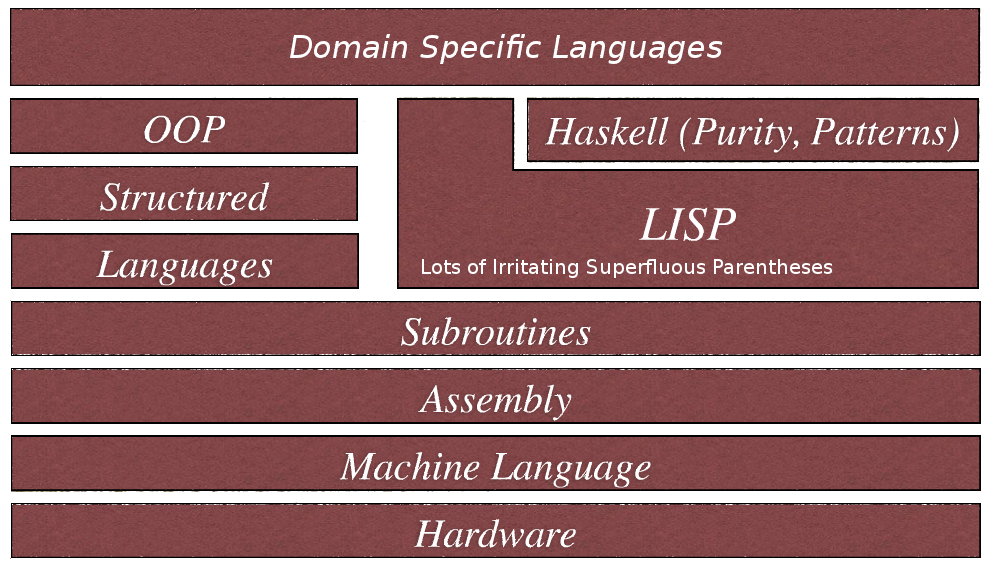
\includegraphics[width=0.9\textwidth]{future.png}
\end{center}
}
%~~~~~~~~~~~~~~~~~~~~~~~~~~~~~~~~~~~~~~~~~~~~~~~~~~~~~~~~~~~~~~~~~~~~~~~~~~
%~~~~~~~~~~~~~~~~~~~~~~~~~~~~~~~~~~~~~~~~~~~~~~~~~~~~~~~~~~~~~~~~~~~~~~~~~~
%~~~~~~~~~~~~~~~~~~~~~~~~~~~~~~~~~~~~~~~~~~~~~~~~~~~~~~~~~~~~~~~~~~~~~~~~~~
\frame{
\ft{Programming paradigms}
\vfill
\begin{center}
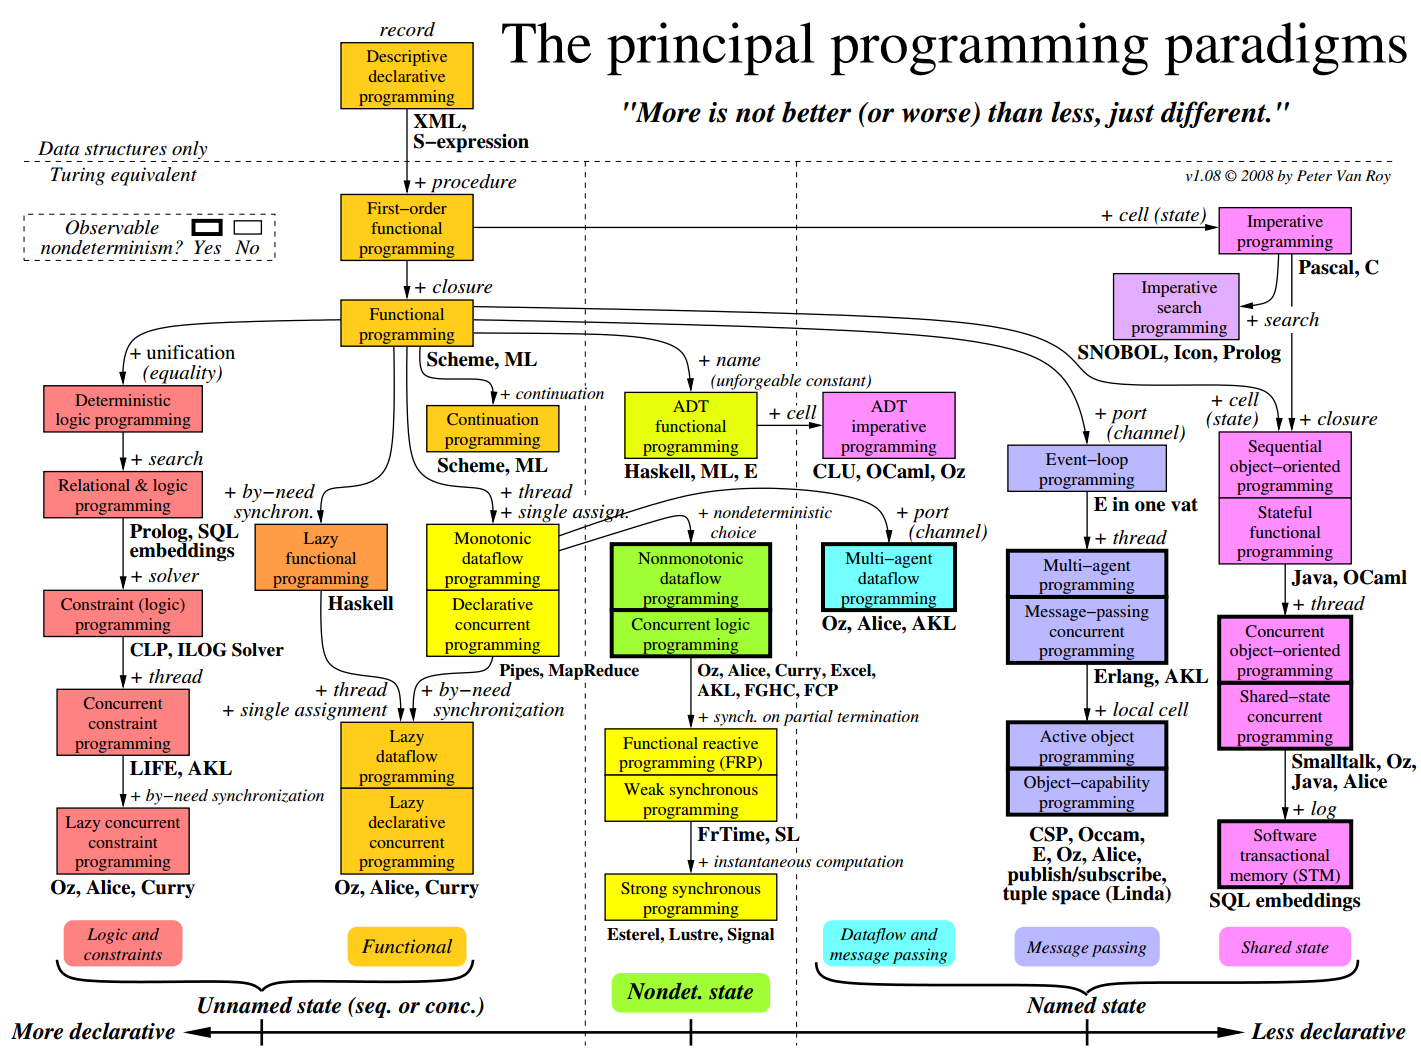
\includegraphics[width=0.9\textwidth]{paradigms.png}
\end{center}
}
%~~~~~~~~~~~~~~~~~~~~~~~~~~~~~~~~~~~~~~~~~~~~~~~~~~~~~~~~~~~~~~~~~~~~~~~~~~
%~~~~~~~~~~~~~~~~~~~~~~~~~~~~~~~~~~~~~~~~~~~~~~~~~~~~~~~~~~~~~~~~~~~~~~~~~~
%~~~~~~~~~~~~~~~~~~~~~~~~~~~~~~~~~~~~~~~~~~~~~~~~~~~~~~~~~~~~~~~~~~~~~~~~~~
\frame{
\ft{Mastering new programming language}
\begin{quote}
''... programming languages are not merely technologies, but habits of mind as well, and nothing changes slower.''\\
\small{--- \textup{Paul Graham}, Beating the Averages}
\end{quote}
}
\section{GSL}
%~~~~~~~~~~~~~~~~~~~~~~~~~~~~~~~~~~~~~~~~~~~~~~~~~~~~~~~~~~~~~~~~~~~~~~~~~~
%~~~~~~~~~~~~~~~~~~~~~~~~~~~~~~~~~~~~~~~~~~~~~~~~~~~~~~~~~~~~~~~~~~~~~~~~~~
%~~~~~~~~~~~~~~~~~~~~~~~~~~~~~~~~~~~~~~~~~~~~~~~~~~~~~~~~~~~~~~~~~~~~~~~~~~
\frame{
\ft{GSL - Advantages and disadvantages}
\bi
\item Easy to learn and use
\item Almost no dependencies - pure C
\item Multiplatform
\item General purpose - not restricted to one model
\item Generated code can be very readable
\item No editor support (vim syntax coloring)
\item XML-driven - complex models not very readable
\item No models defaultly available
\ei 
}
\frame{
\ft{GSL - How does it look like ?}
\vfill
\begin{center}
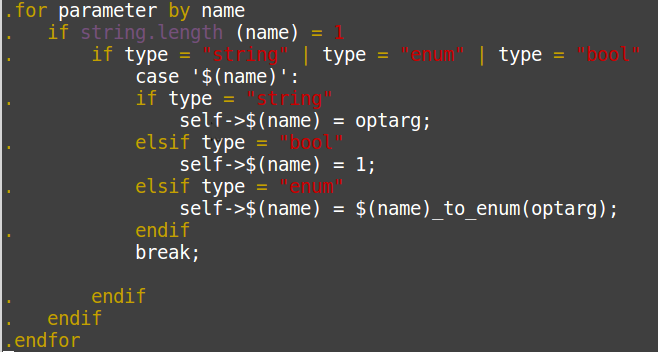
\includegraphics[width=0.8\textwidth]{look.png}
\end{center}
}
%~~~~~~~~~~~~~~~~~~~~~~~~~~~~~~~~~~~~~~~~~~~~~~~~~~~~~~~~~~~~~~~~~~~~~~~~~~
%~~~~~~~~~~~~~~~~~~~~~~~~~~~~~~~~~~~~~~~~~~~~~~~~~~~~~~~~~~~~~~~~~~~~~~~~~~
%~~~~~~~~~~~~~~~~~~~~~~~~~~~~~~~~~~~~~~~~~~~~~~~~~~~~~~~~~~~~~~~~~~~~~~~~~~
\section{Yakindu}
%~~~~~~~~~~~~~~~~~~~~~~~~~~~~~~~~~~~~~~~~~~~~~~~~~~~~~~~~~~~~~~~~~~~~~~~~~~
%~~~~~~~~~~~~~~~~~~~~~~~~~~~~~~~~~~~~~~~~~~~~~~~~~~~~~~~~~~~~~~~~~~~~~~~~~~
%~~~~~~~~~~~~~~~~~~~~~~~~~~~~~~~~~~~~~~~~~~~~~~~~~~~~~~~~~~~~~~~~~~~~~~~~~~
\frame{
\ft{Yakindu - Advantages and disadvantages}
\bi
\item Excellent editor support - model as well as code generator creation
\item Multiplatform - Java
\item Specific - only statechart paradigm
\item Large - many dependencies  
\ei 
}
%~~~~~~~~~~~~~~~~~~~~~~~~~~~~~~~~~~~~~~~~~~~~~~~~~~~~~~~~~~~~~~~~~~~~~~~~~~
%~~~~~~~~~~~~~~~~~~~~~~~~~~~~~~~~~~~~~~~~~~~~~~~~~~~~~~~~~~~~~~~~~~~~~~~~~~
%~~~~~~~~~~~~~~~~~~~~~~~~~~~~~~~~~~~~~~~~~~~~~~~~~~~~~~~~~~~~~~~~~~~~~~~~~~
\frame{
\ft{Yakindu - Xtend2 - syntax and editor support}
\vfill
\begin{center}
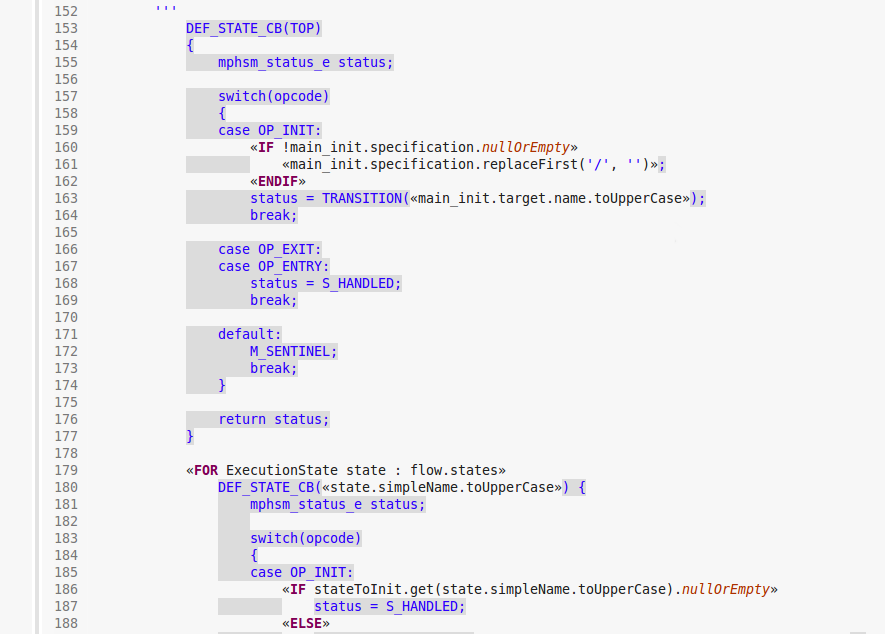
\includegraphics[width=0.9\textwidth]{grayed_2.png}
\end{center}
}
%~~~~~~~~~~~~~~~~~~~~~~~~~~~~~~~~~~~~~~~~~~~~~~~~~~~~~~~~~~~~~~~~~~~~~~~~~~
%~~~~~~~~~~~~~~~~~~~~~~~~~~~~~~~~~~~~~~~~~~~~~~~~~~~~~~~~~~~~~~~~~~~~~~~~~~
%~~~~~~~~~~~~~~~~~~~~~~~~~~~~~~~~~~~~~~~~~~~~~~~~~~~~~~~~~~~~~~~~~~~~~~~~~~
\frame{
\ft{Yakindu - Xtend2 - syntax and editor support}
\vfill
\begin{center}
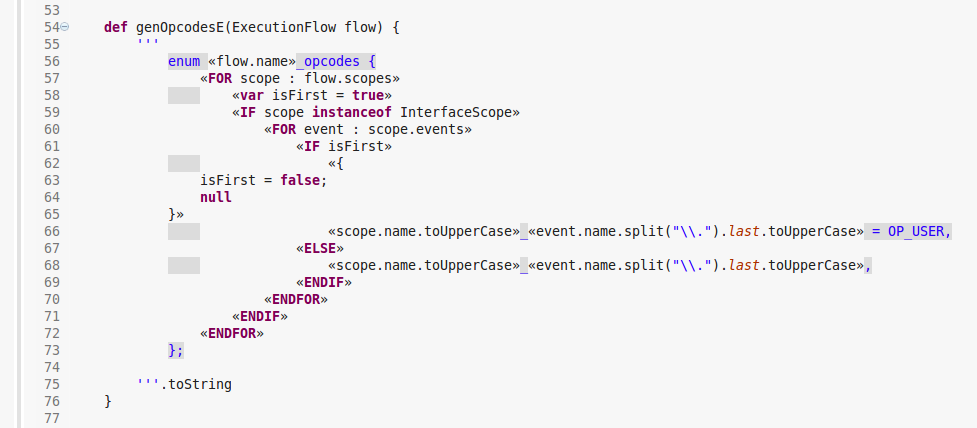
\includegraphics[width=1.0\textwidth]{staircase.png}
\end{center}
}
\section{Atom}
%~~~~~~~~~~~~~~~~~~~~~~~~~~~~~~~~~~~~~~~~~~~~~~~~~~~~~~~~~~~~~~~~~~~~~~~~~~
%~~~~~~~~~~~~~~~~~~~~~~~~~~~~~~~~~~~~~~~~~~~~~~~~~~~~~~~~~~~~~~~~~~~~~~~~~~
%~~~~~~~~~~~~~~~~~~~~~~~~~~~~~~~~~~~~~~~~~~~~~~~~~~~~~~~~~~~~~~~~~~~~~~~~~~
\frame{
\ft{Atom - Advantages and disadvantages}
\bi
\item Allows static analysis and formal verification
\item Very specific - atomic guarded actions paradigm (Bluespec)
\item Multiplatform
\item Designed as Haskell monadic EDSL
\item Pure Haskell syntax
\item Requires understanding of very abstract concepts applicative functors, monoids and monads
\ei 
}

\frame{
\ft{Atom - Enforced restrictions}
\bi
\item Atom designs are always finite state: all variables are global and declared at compile time and dynamic memory allocation is not allowed
\item Atom provides no function or looping constructs. Instead state variable updates are pure combinational functions of the current state.
\ei 
}
%~~~~~~~~~~~~~~~~~~~~~~~~~~~~~~~~~~~~~~~~~~~~~~~~~~~~~~~~~~~~~~~~~~~~~~~~~~
%~~~~~~~~~~~~~~~~~~~~~~~~~~~~~~~~~~~~~~~~~~~~~~~~~~~~~~~~~~~~~~~~~~~~~~~~~~
%~~~~~~~~~~~~~~~~~~~~~~~~~~~~~~~~~~~~~~~~~~~~~~~~~~~~~~~~~~~~~~~~~~~~~~~~~~
\begin{frame}[fragile]
\frametitle{Atom - Syntax}

\begin{semiverbatim}
\begin{lstlisting}
>   period 2000 $ phase 500 $ atom "powerOn" $ do
>     call "sensor_on"
>     triggered <== false
>     ready <== false
>     sensorOn <== true
>     startTimer warmup $ Const 10
>   
>   atom "trigger" $ do
>     cond $ timerDone warmup &&. not_ (value triggered) &&. value sensorOn
>     triggered <== true
>     call "sensor_trigger"
>     
>   atom "checkSensorValue" $ do
>     cond $ value ready
>     ready <== false
>     sensorOn <== false
>     call "sensor_off"
>     atom "checkThreshold" $ do
>       cond $ value sensorValue >. Const threshold
>       overThresholdAction

\end{lstlisting}
\end{semiverbatim}
\end{frame}
\frame{
\ft{Ivory - approach similar to Atom}
\bi
\item DSL embedded into Haskell
\item enforces memory safety and avoids most undefined behaviours while providing low-level control of memory manipulation
\item direct support for model-checking, theorem-proving, and property-based testing
\item concrete C-like syntax for Ivory as a quasi-quoter
\item average case performance (energy efficiency) is often sacrificed in order to bound the worst case
\ei 
}
%~~~~~~~~~~~~~~~~~~~~~~~~~~~~~~~~~~~~~~~~~~~~~~~~~~~~~~~~~~~~~~~~~~~~~~~~~~
%~~~~~~~~~~~~~~~~~~~~~~~~~~~~~~~~~~~~~~~~~~~~~~~~~~~~~~~~~~~~~~~~~~~~~~~~~~
%~~~~~~~~~~~~~~~~~~~~~~~~~~~~~~~~~~~~~~~~~~~~~~~~~~~~~~~~~~~~~~~~~~~~~~~~~~
\frame{
\ft{Ivory - projects}
\bi
\item created and used by DARPA HACMS group (High Assurance Cyber Military Systems)
\item SMACCMPilot - full-featured high-assurance autopilot for a small unpiloted air vehicle
\item Boeing has used Ivory to implement a level-of-interoperability for Stanag 4586, unpiloted air vehicle communications standard
\ei 
}
%~~~~~~~~~~~~~~~~~~~~~~~~~~~~~~~~~~~~~~~~~~~~~~~~~~~~~~~~~~~~~~~~~~~~~~~~~~
%~~~~~~~~~~~~~~~~~~~~~~~~~~~~~~~~~~~~~~~~~~~~~~~~~~~~~~~~~~~~~~~~~~~~~~~~~~
%~~~~~~~~~~~~~~~~~~~~~~~~~~~~~~~~~~~~~~~~~~~~~~~~~~~~~~~~~~~~~~~~~~~~~~~~~~
\frame{
\ft{Ivory - projects}
\vfill
\begin{center}
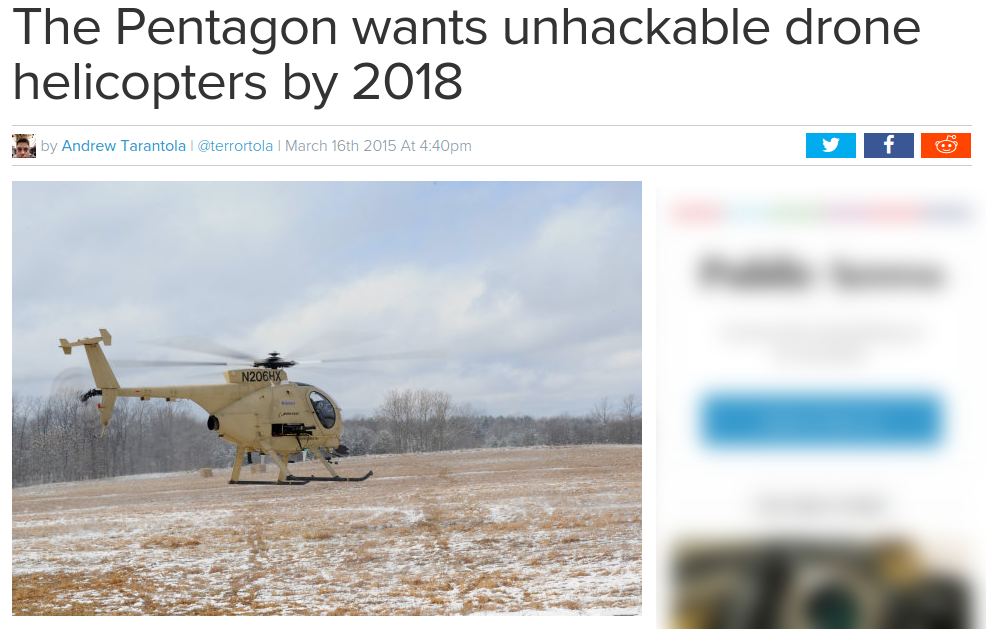
\includegraphics[width=0.9\textwidth]{pentagon.png}
\end{center}
}
%~~~~~~~~~~~~~~~~~~~~~~~~~~~~~~~~~~~~~~~~~~~~~~~~~~~~~~~~~~~~~~~~~~~~~~~~~~
%~~~~~~~~~~~~~~~~~~~~~~~~~~~~~~~~~~~~~~~~~~~~~~~~~~~~~~~~~~~~~~~~~~~~~~~~~~
%~~~~~~~~~~~~~~~~~~~~~~~~~~~~~~~~~~~~~~~~~~~~~~~~~~~~~~~~~~~~~~~~~~~~~~~~~~
\frame{
\ft{Ivory - projects}
\vfill
\begin{center}
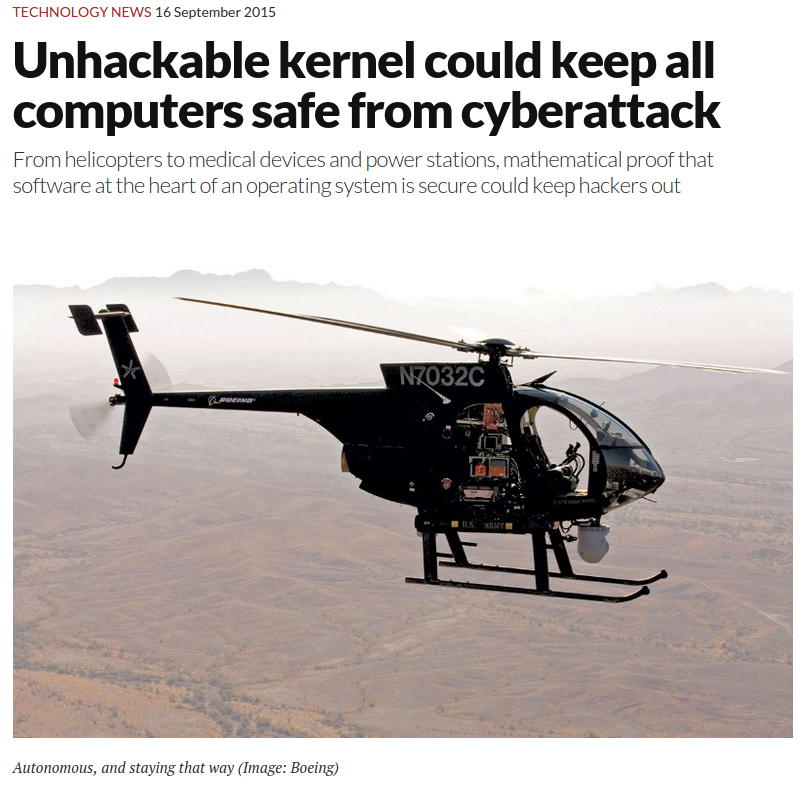
\includegraphics[width=0.8\textwidth]{kernel.png}
\end{center}
}
\section{K}
%~~~~~~~~~~~~~~~~~~~~~~~~~~~~~~~~~~~~~~~~~~~~~~~~~~~~~~~~~~~~~~~~~~~~~~~~~~
%~~~~~~~~~~~~~~~~~~~~~~~~~~~~~~~~~~~~~~~~~~~~~~~~~~~~~~~~~~~~~~~~~~~~~~~~~~
%~~~~~~~~~~~~~~~~~~~~~~~~~~~~~~~~~~~~~~~~~~~~~~~~~~~~~~~~~~~~~~~~~~~~~~~~~~
\frame{
\ft{K-framewrok - matching logic approach}
\bi
\item Define the language grammar in BNF-line notation
\item Get the interpreter, compiler, state-space explorer, model checker for free
\ei 
}
%~~~~~~~~~~~~~~~~~~~~~~~~~~~~~~~~~~~~~~~~~~~~~~~~~~~~~~~~~~~~~~~~~~~~~~~~~~
%~~~~~~~~~~~~~~~~~~~~~~~~~~~~~~~~~~~~~~~~~~~~~~~~~~~~~~~~~~~~~~~~~~~~~~~~~~
%~~~~~~~~~~~~~~~~~~~~~~~~~~~~~~~~~~~~~~~~~~~~~~~~~~~~~~~~~~~~~~~~~~~~~~~~~~
\begin{frame}[fragile]
\frametitle{K - Syntax}

\begin{semiverbatim}
\begin{lstlisting}
> rule [restoreMethContext]:
>     <k> restoreMethContext(MethContext:Bag) => . ...</k>
>     <methodContext> _ => MethContext </methodContext>
> 
> /*@ \subsection{lvalue and loc syntax} */
> 
> syntax KItem ::= lvalue ( K )
> syntax RawVal ::= Loc
> syntax Loc ::= StoreLoc | FieldLoc | ArrayElemLoc
> syntax StoreLoc ::= loc ( Int )
> syntax FieldLoc ::= fieldloc (Int, ClassType, Id) //instance
>                   | fieldloc (ClassType, Id)      //static
> syntax ArrayElemLoc ::= aeloc (Int, Int)

\end{lstlisting}
\end{semiverbatim}
\end{frame}
%~~~~~~~~~~~~~~~~~~~~~~~~~~~~~~~~~~~~~~~~~~~~~~~~~~~~~~~~~~~~~~~~~~~~~~~~~~
%~~~~~~~~~~~~~~~~~~~~~~~~~~~~~~~~~~~~~~~~~~~~~~~~~~~~~~~~~~~~~~~~~~~~~~~~~~
%~~~~~~~~~~~~~~~~~~~~~~~~~~~~~~~~~~~~~~~~~~~~~~~~~~~~~~~~~~~~~~~~~~~~~~~~~~
\frame{
\ft{K - Advantages and disadvantages}
\bi
\item Allows static analysis and formal verification
\item Multiplatform (Java)
\item General purpose - not restricted to one model
\item No editor support
\item No models defaultly available
\item Own specific syntax
\ei 
}
\section{Summary}
%~~~~~~~~~~~~~~~~~~~~~~~~~~~~~~~~~~~~~~~~~~~~~~~~~~~~~~~~~~~~~~~~~~~~~~~~~~
%~~~~~~~~~~~~~~~~~~~~~~~~~~~~~~~~~~~~~~~~~~~~~~~~~~~~~~~~~~~~~~~~~~~~~~~~~~
%~~~~~~~~~~~~~~~~~~~~~~~~~~~~~~~~~~~~~~~~~~~~~~~~~~~~~~~~~~~~~~~~~~~~~~~~~~
\frame{
\ft{Comparison}
\begin{table}
\resizebox{\textwidth}{!}{%
\begin{tabular}{|r|c|c|c|c|c|}
  \hline 
  & Learning curve & Scope & Dependencies & Portable & Editor support\\
  \hline
  GSL & \cellcolor{green!25}short & \cellcolor{green!25}general purpose & \cellcolor{green!25}almost none  & \cellcolor{green!25}yes & \cellcolor{red!25}no \\
  \hline
  Yakindu & \cellcolor{yellow!25}moderate & \cellcolor{yellow!25}specialized & \cellcolor{yellow!25}many & \cellcolor{green!25}yes & \cellcolor{green!25}yes \\
  \hline
  Atom & \cellcolor{red!25}long & \cellcolor{red!25}very specialized & \cellcolor{yellow!25}many & \cellcolor{green!25}yes & \cellcolor{yellow!25}yes/no \\
  \hline
  Ivory & \cellcolor{yellow!25}moderate/long & \cellcolor{yellow!25}specialized & \cellcolor{yellow!25}many & \cellcolor{green!25}yes & \cellcolor{yellow!25}yes/no \\
  \hline
  K & \cellcolor{red!25}long & \cellcolor{green!25}general purpose & \cellcolor{yellow!25}many & \cellcolor{green!25}yes & \cellcolor{red!25}no \\
  \hline
\end{tabular}
}
\end{table}
}
%~~~~~~~~~~~~~~~~~~~~~~~~~~~~~~~~~~~~~~~~~~~~~~~~~~~~~~~~~~~~~~~~~~~~~~~~~~
%~~~~~~~~~~~~~~~~~~~~~~~~~~~~~~~~~~~~~~~~~~~~~~~~~~~~~~~~~~~~~~~~~~~~~~~~~~
%~~~~~~~~~~~~~~~~~~~~~~~~~~~~~~~~~~~~~~~~~~~~~~~~~~~~~~~~~~~~~~~~~~~~~~~~~~
\begin{frame}[allowframebreaks]
        \nocite{*} 
        \frametitle{References}
        \bibliographystyle{amsalpha}
        \bibliography{references}
\end{frame}
%~~~~~~~~~~~~~~~~~~~~~~~~~~~~~~~~~~~~~~~~~~~~~~~~~~~~~~~~~~~~~~~~~~~~~~~~~~
%~~~~~~~~~~~~~~~~~~~~~~~~~~~~~~~~~~~~~~~~~~~~~~~~~~~~~~~~~~~~~~~~~~~~~~~~~~
%~~~~~~~~~~~~~~~~~~~~~~~~~~~~~~~~~~~~~~~~~~~~~~~~~~~~~~~~~~~~~~~~~~~~~~~~~~
\frame{
\begin{center}
\textbf{THE END}

\textbf{Questions?}
\end{center}
}
\end{document}
